% Biên dịch: xelatex bao_cao_cai_tien.tex (chạy hai lần để có mục lục)
\documentclass[12pt,a4paper]{article}
\usepackage{fontspec}
\IfFontExistsTF{Times New Roman}{\setmainfont{Times New Roman}}{\IfFontExistsTF{Liberation Serif}{\setmainfont{Liberation Serif}}{\setmainfont{DejaVu Serif}}}
\IfFontExistsTF{Liberation Mono}{\setmonofont[Scale=0.85]{Liberation Mono}}{\setmonofont[Scale=0.85]{DejaVu Sans Mono}}
\usepackage[margin=2.3cm]{geometry}
\usepackage{booktabs,tabularx,array,graphicx,xcolor,enumitem,float,caption,amssymb}
\usepackage[htt]{hyphenat}
\usepackage[hidelinks]{hyperref}
\sloppy\setlength{\emergencystretch}{3em}
\renewcommand{\contentsname}{Mục lục}
\renewcommand{\tablename}{Bảng}
\renewcommand{\figurename}{Hình}
\setlist{itemsep=2pt,topsep=4pt}
\setlength{\parskip}{5pt}\setlength{\parindent}{0pt}
\newcolumntype{Y}{>{\raggedright\arraybackslash}X}
\newcommand{\code}[1]{\texttt{#1}}

\title{\textbf{Báo cáo cải tiến sản phẩm}\\[4pt]\large ScanGuard / GraphFusionDetect: phát hiện lỗ hổng hợp đồng thông minh\\bằng CodeBERT và mạng nơ-ron đồ thị}
\author{Vòng chung kết cuộc thi Sáng tạo trẻ Quốc gia\\trong lĩnh vực Trí tuệ nhân tạo năm 2026}
\date{Tháng 11 năm 2026}

\begin{document}
\maketitle

\section*{Tóm tắt}
Báo cáo trình bày kết quả thực hiện ba yêu cầu cải tiến của ban tổ chức đối với hai loại lỗ hổng mà sản phẩm hỗ trợ: phụ thuộc thời gian khối (timestamp dependency) và tái nhập (reentrancy).
\begin{itemize}
\item \textbf{Yêu cầu 1.} Trên cùng tập kiểm thử và cùng máy, mô hình GFD đạt macro-F1 0{,}85 (timestamp) và 0{,}73 (reentrancy), cao hơn công cụ phân tích tĩnh Slither (0{,}75 và 0{,}62). Thành phần ngữ nghĩa, đặc biệt là bước fine-tune CodeBERT theo từng lỗ hổng, là nguồn cải thiện có ý nghĩa thống kê.
\item \textbf{Yêu cầu 2.} Trên dự án chưa thấy, hợp đồng lớn, mã đối kháng và ca khó có nhãn chuyên gia, mô hình bộc lộ giới hạn rõ ràng về bỏ sót và cảnh báo nhầm. Báo cáo nêu nguyên nhân từng nhóm lỗi và một biện pháp khắc phục đã triển khai (loại comment trước khi mã hoá).
\item \textbf{Yêu cầu 3.} Sản phẩm quét song song hai lỗ hổng, đưa bằng chứng theo dòng mã vào IDE và CI (SARIF), và thực thi ở máy chủ quy trình phát hiện $\rightarrow$ giải thích $\rightarrow$ chuyên gia xác nhận $\rightarrow$ sửa $\rightarrow$ biên dịch và kiểm tra lại $\rightarrow$ chuyên gia duyệt. Sản phẩm không khẳng định hợp đồng an toàn ở bất kỳ bước nào.
\end{itemize}
Mọi số liệu trong báo cáo được sinh từ mã và kết quả thô đi kèm trong kho mã (thư mục \code{eval/} và \code{demo/}).

\tableofcontents
\newpage

\section{Bối cảnh và thiết lập chung}
\subsection{Kiến trúc được đánh giá}
Với mỗi hợp đồng, sản phẩm dùng Slither để dựng đồ thị gọi hàm, dùng CodeBERT đã fine-tune theo từng lỗ hổng để mã hoá mỗi hàm thành một vector 768 chiều, rồi dùng hai mạng nơ-ron đồ thị: một mạng phân loại cả hợp đồng và một mạng phân loại từng hàm. Mỗi lỗ hổng có bộ ba mô hình riêng (Bảng~\ref{tab:models}).

\begin{table}[H]\centering\small
\caption{Bộ ba mô hình của từng lỗ hổng.}\label{tab:models}
\begin{tabularx}{\textwidth}{lYY}
\toprule
 & Timestamp dependency & Reentrancy\\
\midrule
Bộ mã hoá hàm & \code{codebert-solidity-time-dep} & \code{codebert-solidity-re-entrancy}\\
Mô hình mức hợp đồng & GCN 2 lớp (2048), max pooling & GAT 2 lớp (2048), max pooling, 2 lớp liên hợp đồng\\
Mô hình mức hàm & GAT (256, 128) & GAT (256, 128)\\
\bottomrule
\end{tabularx}
\end{table}

\subsection{Dữ liệu, phần cứng và khả năng tái hiện}
\begin{itemize}
\item \textbf{Dữ liệu huấn luyện và kiểm thử chuẩn:} bộ dữ liệu của bài báo, đã loại trùng hàm giữa hai tập, giữ nguyên cách chia. Timestamp: 807 hợp đồng huấn luyện, 193 kiểm thử. Reentrancy: 611 huấn luyện, 147 kiểm thử.
\item \textbf{Phần cứng:} GPU NVIDIA L40S (46 GB), CPU Intel Xeon Gold 6542Y, 32 luồng. Mọi hệ thống trong cùng một bảng chạy trên cùng máy này.
\item \textbf{Phần mềm:} PyTorch 2.4.0, DGL 2.4.0 (CUDA 12.1), Slither 0.8.0, trình biên dịch solc chọn theo \code{pragma} của từng hợp đồng.
\item \textbf{Tái hiện:} \code{eval/ablation/run\_all.sh} (yêu cầu 1), \code{eval/generalization/run\_all.sh} và \code{report.py} (yêu cầu 2), \code{demo/run\_demo.py} (yêu cầu 3). Phiên bản thư viện ghi trong \code{eval/ablation/requirements-gpu.txt}.
\end{itemize}

\section{Yêu cầu 1: Chứng minh đóng góp của kiến trúc kết hợp}
\subsection{Thiết kế thí nghiệm}
Bốn hệ thống được so sánh trên cùng tập kiểm thử:
\begin{itemize}
\item \textbf{GFD đầy đủ:} CodeBERT fine-tune theo lỗ hổng, đồ thị gọi hàm và GNN.
\item \textbf{Bỏ ngữ nghĩa:} giữ đồ thị và GNN; mỗi hàm chỉ còn 5 đặc trưng cấu trúc (bậc vào, bậc ra, Katz, closeness, hệ số phân cụm).
\item \textbf{Ngữ nghĩa chưa fine-tune:} như GFD đầy đủ nhưng vector hàm lấy từ \code{microsoft/codebert-base}.
\item \textbf{Slither 0.8.0:} công cụ phân tích tĩnh, dùng detector của chính nó cho từng lỗ hổng.
\end{itemize}
Để so sánh công bằng, mọi biến thể học máy được huấn luyện lại theo cùng một quy trình: siêu tham số theo notebook của nhóm, tối ưu Adam, seed 42, tách 20\% tập huấn luyện làm tập validation và chọn epoch theo macro-F1 trên validation, không dùng tập kiểm thử để chọn. Hợp đồng được chấm từng cái một, đúng cách API của sản phẩm hoạt động. Chỉ những hợp đồng mà mọi hệ thống đều chấm được mới được tính (187/193 và 144/147). Ý nghĩa thống kê được kiểm bằng kiểm định McNemar chính xác hai phía so với GFD đầy đủ.

\subsection{Kết quả theo từng lớp}
\begin{table}[H]\centering\small
\caption{Timestamp dependency: 187 hợp đồng kiểm thử (96 có lỗi). P, R, F1 theo từng lớp.}\label{tab:ts}
\setlength{\tabcolsep}{4pt}
\begin{tabular}{lccccccccc}
\toprule
 & \multicolumn{3}{c}{Lớp không lỗi} & \multicolumn{3}{c}{Lớp có lỗi} & & & \\
\cmidrule(lr){2-4}\cmidrule(lr){5-7}
Hệ thống & P & R & F1 & P & R & F1 & Macro-F1 & Acc. & $p$ McNemar\\
\midrule
GFD đầy đủ & 0{,}83 & 0{,}87 & 0{,}85 & 0{,}87 & 0{,}83 & 0{,}85 & \textbf{0{,}85} & 0{,}85 & --\\
Bỏ ngữ nghĩa & 0{,}78 & 0{,}70 & 0{,}74 & 0{,}74 & 0{,}81 & 0{,}78 & 0{,}76 & 0{,}76 & 0{,}010\\
Ngữ nghĩa chưa fine-tune & 0{,}75 & 0{,}86 & 0{,}80 & 0{,}84 & 0{,}73 & 0{,}78 & 0{,}79 & 0{,}79 & 0{,}027\\
Slither (\code{timestamp}) & 0{,}75 & 0{,}73 & 0{,}74 & 0{,}75 & 0{,}77 & 0{,}76 & 0{,}75 & 0{,}75 & 0{,}007\\
\bottomrule
\end{tabular}
\end{table}

\begin{table}[H]\centering\small
\caption{Reentrancy: 144 hợp đồng kiểm thử (71 có lỗi).}\label{tab:re}
\setlength{\tabcolsep}{4pt}
\begin{tabular}{lccccccccc}
\toprule
 & \multicolumn{3}{c}{Lớp không lỗi} & \multicolumn{3}{c}{Lớp có lỗi} & & & \\
\cmidrule(lr){2-4}\cmidrule(lr){5-7}
Hệ thống & P & R & F1 & P & R & F1 & Macro-F1 & Acc. & $p$ McNemar\\
\midrule
GFD đầy đủ & 0{,}81 & 0{,}63 & 0{,}71 & 0{,}69 & 0{,}85 & 0{,}76 & \textbf{0{,}73} & 0{,}74 & --\\
Bỏ ngữ nghĩa & 0{,}66 & 0{,}77 & 0{,}71 & 0{,}71 & 0{,}59 & 0{,}65 & 0{,}68 & 0{,}68 & 0{,}350\\
Ngữ nghĩa chưa fine-tune & 0{,}76 & 0{,}43 & 0{,}54 & 0{,}59 & 0{,}86 & 0{,}70 & 0{,}62 & 0{,}64 & 0{,}034\\
Slither (mọi \code{reentrancy-*}) & 0{,}80 & 0{,}27 & 0{,}41 & 0{,}56 & 0{,}93 & 0{,}70 & 0{,}55 & 0{,}60 & 0{,}003\\
Slither (\code{reentrancy-eth}) & 0{,}60 & 0{,}81 & 0{,}69 & 0{,}70 & 0{,}45 & 0{,}55 & 0{,}62 & 0{,}63 & 0{,}072\\
\bottomrule
\end{tabular}
\end{table}

Khi loại các hợp đồng gần trùng nhau (cùng nhãn, cùng số hàm, cùng số cạnh), thứ tự các hệ thống không đổi: macro-F1 của GFD đầy đủ là 0{,}84 trên 156 hợp đồng timestamp và 0{,}73 trên 123 hợp đồng reentrancy.

\subsection{Mức đóng góp của từng thành phần}
\begin{itemize}
\item \textbf{Ngữ nghĩa.} Bỏ vector CodeBERT làm macro-F1 giảm 9 điểm ở timestamp ($p = 0{,}010$) và 6 điểm ở reentrancy ($p = 0{,}35$, chưa đạt ý nghĩa thống kê).
\item \textbf{Bước fine-tune theo lỗ hổng.} Thay bằng CodeBERT gốc làm giảm 6 điểm ở timestamp ($p = 0{,}027$) và 11 điểm ở reentrancy ($p = 0{,}034$). Ở reentrancy, CodeBERT gốc còn kém bản chỉ dùng đặc trưng cấu trúc: embedding mã nguồn tổng quát không tự mang lại lợi ích, chính bước fine-tune mới tạo ra giá trị.
\item \textbf{So với phân tích tĩnh.} GFD hơn Slither 10 điểm ở timestamp ($p = 0{,}007$). Ở reentrancy, GFD hơn 18 điểm so với tập hợp mọi detector \code{reentrancy-*} ($p = 0{,}003$) và 11 điểm so với \code{reentrancy-eth} ($p = 0{,}072$).
\item \textbf{Tính chất lỗi khác nhau.} Với reentrancy, Slither dùng mọi detector có recall lớp có lỗi 0{,}93 nhưng recall lớp không lỗi chỉ 0{,}27; GFD cân bằng hơn (0{,}85 và 0{,}63).
\end{itemize}

\subsection{Thời gian và tài nguyên}
\begin{table}[H]\centering\small
\caption{Chi phí huấn luyện và suy luận.}\label{tab:cost}
\begin{tabular}{lcc}
\toprule
 & Timestamp & Reentrancy\\
\midrule
Số tham số GNN mức hợp đồng & 6{,}3 triệu & 55{,}1 triệu\\
Số hợp đồng dùng để huấn luyện (sau khi tách validation) & 610 & 452\\
Thời gian huấn luyện GNN (GFD đầy đủ) & 31 giây & 93 giây\\
Bộ nhớ GPU đỉnh khi huấn luyện & 0{,}46 GB & 4{,}4 GB\\
Dựng đồ thị và mã hoá hàm, trung vị mỗi hợp đồng & 0{,}65 giây & 0{,}36 giây\\
Suy luận GNN, mỗi hợp đồng & 2{,}5 ms & 6{,}4 ms\\
Slither, trung vị mỗi hợp đồng & 0{,}28 giây & 0{,}23 giây\\
\bottomrule
\end{tabular}
\end{table}
GFD chậm hơn Slither khoảng 1{,}5 đến 2{,}3 lần cho mỗi hợp đồng; gần như toàn bộ thời gian nằm ở bước dựng đồ thị và mã hoá hàm, bước này dùng chung cho mọi biến thể.

\subsection{Phân tích trường hợp cải thiện và suy giảm}
Bảng~\ref{tab:cases} chọn bảy hợp đồng trong tập kiểm thử mà GFD đầy đủ kết luận đúng, và cho thấy mỗi phương pháp còn lại đúng ở trường hợp này nhưng sai ở trường hợp khác. Dấu \checkmark{} là kết luận đúng với nhãn, dấu $\times$ là sai.

\begin{table}[H]\centering\small
\caption{Bảy hợp đồng GFD kết luận đúng; các phương pháp khác lúc đúng lúc sai.}\label{tab:cases}
\begin{tabularx}{\textwidth}{clYlcccc}
\toprule
\# & Lỗ hổng & Hợp đồng (thư mục Test) & Nhãn & GFD & Bỏ ngữ nghĩa & CodeBERT gốc & Slither\\
\midrule
1 & timestamp & \code{0xde29\ldots0d99.sol} & không lỗi & \checkmark & $\times$ & \checkmark & \checkmark\\
2 & timestamp & \code{0x57f8\ldots1932.sol} & có lỗi & \checkmark & \checkmark & $\times$ & \checkmark\\
3 & timestamp & \code{0x98c1\ldots3cd8.sol} & có lỗi & \checkmark & \checkmark & \checkmark & $\times$\\
4 & reentrancy & \code{0x6805\ldots9fd0.sol} & không lỗi & \checkmark & $\times$ & \checkmark & \checkmark\\
5 & reentrancy & \code{0xc8d9\ldots b611.sol} & không lỗi & \checkmark & $\times$ & $\times$ & \checkmark\\
6 & reentrancy & \code{0x6091\ldots3b36.sol} & không lỗi & \checkmark & \checkmark & \checkmark & $\times$\\
7 & reentrancy & \code{0x98fe\ldots0377.sol} & có lỗi & \checkmark & $\times$ & $\times$ & $\times$\\
\bottomrule
\end{tabularx}
\end{table}
Slither ở các dòng reentrancy là detector \code{reentrancy-eth}.
\begin{enumerate}
\item \textbf{Bỏ ngữ nghĩa suy giảm.} Hợp đồng chỉ dùng \code{block.timestamp / (1 days)} làm tham số của một sự kiện log (dòng 25 và 29). Bản chỉ có đặc trưng cấu trúc báo lỗi vì không đọc được nội dung hàm; các hệ thống còn lại kết luận đúng.
\item \textbf{CodeBERT gốc suy giảm.} Trong hợp đồng \code{Presale}, \code{now} nằm ở hàm phụ \code{presaleOpen()} (dòng 65--66), quyết định việc nhận tiền ở hàm fallback (dòng 50). CodeBERT chưa fine-tune bỏ sót; GFD và Slither phát hiện.
\item \textbf{Slither suy giảm.} Hàm \code{addRecord} ghi \code{Reb.time = block.timestamp} (dòng 16) vào trạng thái. Detector của Slither chỉ bắt các phép so sánh với thời gian khối nên không báo; ba biến thể học máy đều phát hiện đúng theo nhãn.
\item \textbf{Bỏ ngữ nghĩa suy giảm.} Dòng 12 viết \code{msg.sender.call.value(this.balance);} nhưng thiếu cặp ngoặc gọi hàm, nên không có lời gọi ngoài nào được thực hiện. Bản bỏ ngữ nghĩa báo lỗi; các hệ thống còn lại kết luận đúng.
\item \textbf{Cả hai biến thể ablation suy giảm.} Hàm \code{split} (dòng 8--16) chỉ chuyển tiếp \code{msg.value} tới địa chỉ đích bằng \code{call.value}, không giữ số dư của người dùng nên không có trạng thái để tái nhập khai thác. Bản bỏ ngữ nghĩa và CodeBERT gốc đều báo nhầm; GFD và Slither đúng.
\item \textbf{Slither suy giảm (báo nhầm).} \code{tryExec} (dòng 3--8) là hàm \code{internal} bọc \code{target.call.value(value)(calldata)} của một thư viện thực thi lệnh. \code{reentrancy-eth} báo lỗi; cả ba biến thể học máy kết luận không lỗi, đúng với nhãn.
\item \textbf{Chỉ GFD đúng.} Hàm \code{call} (dòng 34--37) thực hiện \code{addr.call.value(amount)(data)} với địa chỉ và dữ liệu do người gọi truyền vào. \code{reentrancy-eth} không báo vì sau lời gọi không có ghi trạng thái; bản bỏ ngữ nghĩa và CodeBERT gốc cũng bỏ sót.
\end{enumerate}

\textbf{Tổng hợp trên toàn bộ tập kiểm thử.} Bảng~\ref{tab:cases} là các trường hợp được chọn, không phải toàn cảnh; số liệu đầy đủ như sau.
\begin{table}[H]\centering\small
\caption{Số hợp đồng mà GFD và từng phương pháp bất đồng về đúng/sai.}\label{tab:disagree}
\begin{tabular}{lcccc}
\toprule
 & \multicolumn{2}{c}{Timestamp (187)} & \multicolumn{2}{c}{Reentrancy (144)}\\
\cmidrule(lr){2-3}\cmidrule(lr){4-5}
So với GFD & GFD đúng, & GFD sai, & GFD đúng, & GFD sai,\\
 & phương pháp sai & phương pháp đúng & phương pháp sai & phương pháp đúng\\
\midrule
Bỏ ngữ nghĩa & 28 & 11 & 32 & 24\\
CodeBERT gốc & 16 & 5 & 26 & 12\\
Slither & 32 & 13 & 38 & 23\\
\bottomrule
\end{tabular}
\end{table}
GFD kết luận sai 28/187 hợp đồng timestamp và 38/144 hợp đồng reentrancy. Một ví dụ: \code{simple\_dao\_fixed.sol} đã trừ số dư trước khi gọi \code{call.value}, nhưng cả ba biến thể học máy vẫn báo lỗi còn Slither thì không, vì mô hình nhận ra sự có mặt của \code{call.value} chứ không nhận ra thứ tự câu lệnh. Đây là lý do sản phẩm yêu cầu chuyên gia xác nhận ở yêu cầu 3.

\subsection{Giới hạn}
Mỗi biến thể chạy một seed, nên các chênh lệch 2--3 điểm không nên diễn giải. Chỉ so với một công cụ phân tích tĩnh. Bảng đánh giá ở mức hợp đồng, không đánh giá việc định vị hàm. 6 hợp đồng timestamp và 3 hợp đồng reentrancy bị loại vì không biên dịch được.

\section{Yêu cầu 2: Kiểm thử khả năng khái quát và ca khó}
\subsection{Bộ kiểm thử và nguồn đánh giá chuyên môn}
\begin{table}[H]\centering\small
\caption{Bốn nhóm kiểm thử.}\label{tab:sets}
\begin{tabularx}{\textwidth}{lYY}
\toprule
Nhóm & Nguồn mã & Nguồn nhãn chuyên môn\\
\midrule
Dự án chưa thấy & DAppSCAN (IEEE TSE 2024): 36 file timestamp, 114 file reentrancy từ các dự án DApp đã audit & Báo cáo audit của các công ty bảo mật, có tên hàm và số dòng (65 và 138 vị trí)\\
Hợp đồng lớn & Cùng bộ DAppSCAN, chia theo số dòng sau khi gộp file & Như trên\\
Mã đối kháng & 80 hợp đồng kiểm thử mỗi lỗ hổng, biến đổi giữ nguyên ngữ nghĩa & Nhãn gốc (ngữ nghĩa không đổi nên nhãn không đổi)\\
Ca dương và âm khó & Consolidated Ground Truth (TU Wien, 2023): 60 hợp đồng timestamp, 32 hợp đồng reentrancy & Nhãn gán tay của các nhóm nghiên cứu gốc, đã được rà soát hợp nhất\\
\bottomrule
\end{tabularx}
\end{table}
Ca âm khó là hợp đồng được chuyên gia xác nhận không có lỗ hổng nhưng có chứa cú pháp nhạy cảm (\code{now}, \code{block.timestamp}, \code{call.value}). Mọi hợp đồng đi qua đúng các bước của sản phẩm. Kết quả từng ca kèm tên file, hàm và vị trí dòng nằm trong \code{eval/generalization/results\_dappscan.md}, \code{results\_hard.md} và \code{results\_adversarial.md}; bộ mã nằm trong \code{eval/dappscan/flat/} và \code{eval/generalization/}.

\subsection{Dự án chưa thấy}
\begin{table}[H]\centering\small
\caption{Kết quả trên DAppSCAN so với vị trí do auditor chỉ ra.}\label{tab:dapp}
\begin{tabular}{lcc}
\toprule
 & Timestamp & Reentrancy\\
\midrule
Số file / số file dựng được đồ thị & 36 / 17 & 114 / 71\\
Riêng Solidity 0.8: dựng được đồ thị & 7/15 & 21/30\\
Tỉ lệ hàm trùng nguyên văn với tập huấn luyện & 15{,}3\% & 4{,}2\%\\
Số vị trí audit & 65 & 138\\
\quad nằm trong file không dựng được đồ thị & 36 & 53\\
\quad phát hiện đúng hàm & 6 & 1\\
\quad hàm bị gắn cờ nhưng hợp đồng bị xếp không lỗi & 8 & 0\\
\quad bỏ sót & 12 & 83\\
\quad dòng nằm ngoài mọi hàm & 3 & 1\\
\bottomrule
\end{tabular}
\end{table}
\textbf{Ví dụ phát hiện đúng.} \code{wHakka.unstake}: audit chỉ dòng 580, mô hình gắn cờ hàm ở dòng 578--595 với xác suất 1{,}00. \code{Sliced.sendTokens}: audit chỉ dòng 72, mô hình gắn cờ đúng hàm. \code{OrderBook.cancelExpiredOrders}: audit chỉ dòng 145, mô hình gắn cờ với xác suất 0{,}90.

\textbf{Phân tích bỏ sót.}
\begin{itemize}
\item \textbf{Rào cản đầu tiên là dựng đồ thị.} 62/150 file không dựng được: bộ dữ liệu thiếu file import (33), sản phẩm chọn bản solc thấp nhất thoả \code{pragma} (13), file gộp không biên dịch (10), Slither 0.8.0 lỗi sau khi biên dịch được (5), thiếu bản solc (1).
\item \textbf{Mô hình mức hợp đồng chặn mô hình mức hàm.} Ở timestamp, 8 vị trí được mô hình mức hàm gắn cờ đúng nhưng không hiển thị vì hợp đồng bị xếp không lỗi (ví dụ hợp đồng \code{SamuraiLegendsStaking}).
\item \textbf{Reentrancy gần như không khái quát.} Chỉ 2/71 hợp đồng bị gắn cờ. Dữ liệu huấn luyện định nghĩa reentrancy qua cú pháp \code{call.value(...)} của Solidity 0.4; mã từ 0.6 trở lên viết \code{call\{value: ...\}} hoặc gọi qua interface, nên mô hình không nhận ra. Phạm vi áp dụng hiện tại của mô hình reentrancy là mã kiểu Solidity 0.4 và 0.5.
\end{itemize}

\subsection{Hợp đồng lớn}
\begin{table}[H]\centering\small
\caption{Reentrancy trên DAppSCAN, chia theo kích thước file sau khi gộp.}\label{tab:size}
\begin{tabular}{lcccccc}
\toprule
Kích thước & File & Dựng được & Số hàm & Giây/file & Hàm dài hơn & Vị trí audit\\
 & & đồ thị & (trung vị) & (trung vị / lớn nhất) & 512 token & tìm được\\
\midrule
Dưới 500 dòng & 18 & 9 & 29 & 1{,}0 / 3{,}3 & 3/323 & 1/9\\
500--2.000 dòng & 62 & 46 & 95 & 2{,}1 / 8{,}1 & 90/4.583 & 0/59\\
Trên 2.000 dòng & 34 & 16 & 220 & 6{,}9 / 51{,}7 & 126/4.979 & 0/17\\
\bottomrule
\end{tabular}
\end{table}
Thời gian tăng theo số hàm nhưng vẫn ở mức chấp nhận được. Khoảng 2--3\% số hàm dài hơn giới hạn 512 token của CodeBERT và bị cắt khi mã hoá. Với timestamp, nhóm 500--2.000 dòng tìm được 5/24 vị trí audit, nhóm trên 2.000 dòng 0/2.

\subsection{Mã đối kháng}
Năm phép biến đổi giữ nguyên ngữ nghĩa được áp dụng lên các hợp đồng mà mô hình vốn xếp đúng: đổi tên hàm, chèn comment dài ở đầu hàm, chèn mã chết, thêm một hợp đồng mồi nhử chỉ nhắc từ khoá trong comment, và đọc thời gian qua một hàm thư viện.
\begin{table}[H]\centering\small
\caption{Số hợp đồng đổi kết luận sau biến đổi.}\label{tab:adv}
\begin{tabular}{llcc}
\toprule
Lỗ hổng & Phép biến đổi & Có lỗi $\rightarrow$ bị bỏ sót & Không lỗi $\rightarrow$ bị cảnh báo\\
\midrule
Timestamp & Đổi tên hàm & 0/34 & 2/32\\
 & Chèn comment dài & 11/33 & 0/7\\
 & Chèn mã chết & 0/27 & 0/6\\
 & Mồi nhử trong comment & 0/35 & 26/32\\
 & Đọc thời gian qua hàm thư viện & 0/17 & 13/14\\
\midrule
Reentrancy & Chèn comment dài & 17/33 & 0/31\\
 & Chèn mã chết & 7/19 & 0/29\\
 & Mồi nhử trong comment & 0/33 & 0/31\\
\bottomrule
\end{tabular}
\end{table}
\begin{itemize}
\item \textbf{Chèn comment dài} che được lỗi ở cả hai mô hình: comment đẩy dòng nguy hiểm ra ngoài 512 token được mã hoá. Số hàm bị gắn cờ giảm từ 64 xuống 9 (timestamp) và từ 40 xuống 3 (reentrancy).
\item \textbf{Mồi nhử} làm mô hình timestamp cảnh báo nhầm 26/32 hợp đồng không lỗi; hàm mồi bị gắn cờ trong cả 67 hợp đồng. Mô hình timestamp phản ứng với sự xuất hiện của từ khoá, kể cả trong comment.
\item \textbf{Đổi tên hàm} gần như không ảnh hưởng. Chèn mã chết không ảnh hưởng timestamp nhưng làm reentrancy bỏ sót 7/19.
\end{itemize}

\subsection{Ca dương và ca âm khó}
\begin{table}[H]\centering\small
\caption{Kết quả trên bộ CGT có nhãn gán tay.}\label{tab:hard}
\begin{tabular}{lcc}
\toprule
 & Timestamp & Reentrancy\\
\midrule
Ca dương được phát hiện & 29/30 & 3/14\\
Ca âm khó bị cảnh báo nhầm & 27/28 & 6/15\\
Precision / Recall & 0{,}52 / 0{,}97 & 0{,}33 / 0{,}21\\
\bottomrule
\end{tabular}
\end{table}
Với hợp đồng có dùng thời gian khối, mô hình timestamp gần như luôn báo lỗi: recall cao nhưng khả năng phân biệt thấp. Ví dụ cảnh báo nhầm: hàm \code{IcoContract.createTokens} (dòng 281--306, địa chỉ \code{0x52e3\ldots07d5}) bị gắn cờ với xác suất 1{,}00 dù nhãn chuyên gia là không lỗi. Với reentrancy, các ca dương từ bộ Zeus (4/4) và Doublade (3/4) bị bỏ sót.

\subsection{Biện pháp khắc phục đã triển khai}
Từ kết quả đối kháng, sản phẩm đã được sửa để loại comment khỏi mã hàm trước khi đưa vào CodeBERT. Mã hiển thị cho người dùng (trong IDE và danh sách hàm) vẫn giữ nguyên comment và số dòng. Không cần huấn luyện lại.
\begin{table}[H]\centering\small
\caption{Trước và sau khi loại comment (cùng bộ đối kháng).}\label{tab:fix}
\begin{tabular}{lcc}
\toprule
 & Trước & Sau\\
\midrule
Timestamp: tập kiểm thử gốc xếp đúng & 168/187 & 167/187\\
Timestamp: comment dài, ca có lỗi bị bỏ sót & 11/33 & 0/33\\
Timestamp: mồi nhử, ca không lỗi bị cảnh báo & 26/32 & 0/32\\
Reentrancy: mẫu kiểm thử gốc xếp đúng & 64/80 & 64/80\\
Reentrancy: comment dài, ca có lỗi bị bỏ sót & 17/33 & 1/33\\
\bottomrule
\end{tabular}
\end{table}
Hai hướng khắc phục còn lại đã xác định nhưng chưa triển khai: chọn bản solc cao nhất thoả \code{pragma} (cứu được tối đa 13 file DAppSCAN), và bổ sung dữ liệu reentrancy có cú pháp \code{call\{value: ...\}} trước khi tuyên bố hỗ trợ Solidity từ 0.6.

\subsection{Giới hạn của phép thử}
Bộ đối kháng và bộ CGT là mẫu nhỏ nên các tỉ lệ nên được đọc như chỉ báo. Nhãn DAppSCAN chỉ có ca dương, nên không tính precision ở mức hàm. \emph{Phát hiện đúng hàm} nghĩa là hàm bị gắn cờ chứa dòng auditor chỉ ra; mô hình không chỉ tới từng dòng. Bộ CGT có 45\% (timestamp) và 66\% (reentrancy) số hàm trùng với tập huấn luyện do dùng chung thư viện, nên không hoàn toàn là dữ liệu chưa thấy.

\section{Yêu cầu 3: Quy trình sửa lỗi có người xác nhận}
\subsection{Nguyên tắc}
Kết quả ở yêu cầu 1 và 2 cho thấy cả cảnh báo lẫn việc không có cảnh báo đều không đủ để kết luận về an toàn. Vì vậy sản phẩm coi đầu ra của mô hình là manh mối cho con người, và mọi bước quyết định đều do chuyên gia thực hiện. Giao diện, bản xuất SARIF và lời giải thích của mô hình ngôn ngữ đều ghi rõ: cảnh báo cần chuyên gia xác nhận, và hợp đồng không bị cảnh báo vẫn cần audit thủ công.

\subsection{Luồng quét song song và kết luận}
Khi một hợp đồng được tải lên hoặc lấy về theo địa chỉ token, hai luồng quét (timestamp và reentrancy) chạy đồng thời, mỗi luồng gồm: dựng đồ thị, mô hình mức hợp đồng, mô hình mức hàm, giải thích. Kết quả được truyền dần về giao diện, và luồng kết thúc bằng một kết luận chung.
\begin{table}[H]\centering\small
\caption{Trạng thái của từng luồng quét và kết luận chung.}\label{tab:status}
\begin{tabularx}{\textwidth}{lY}
\toprule
Trạng thái luồng & Ý nghĩa\\
\midrule
Bị gắn cờ & Hợp đồng bị cảnh báo và có hàm được định vị\\
Bị gắn cờ, chưa định vị hàm & Hợp đồng bị cảnh báo nhưng không chỉ ra được hàm: chuyển rà soát thủ công\\
Không bị gắn cờ & Không có cảnh báo; không phải bằng chứng an toàn\\
Quét thất bại & Không chạy được (thường do không biên dịch được): chuyển rà soát thủ công\\
\midrule
Kết luận chung & Có cảnh báo, nếu ít nhất một luồng gắn cờ; cần rà soát thủ công, nếu không luồng nào gắn cờ nhưng có luồng thất bại; không có cảnh báo, nếu mọi luồng chạy xong và không gắn cờ\\
\bottomrule
\end{tabularx}
\end{table}
Một luồng lỗi không che kết quả của luồng kia. Giao diện chỉ hiển thị chi tiết cho lỗ hổng có hàm bị gắn cờ; khối kết luận luôn liệt kê trạng thái của cả hai.

\begin{figure}[H]\centering
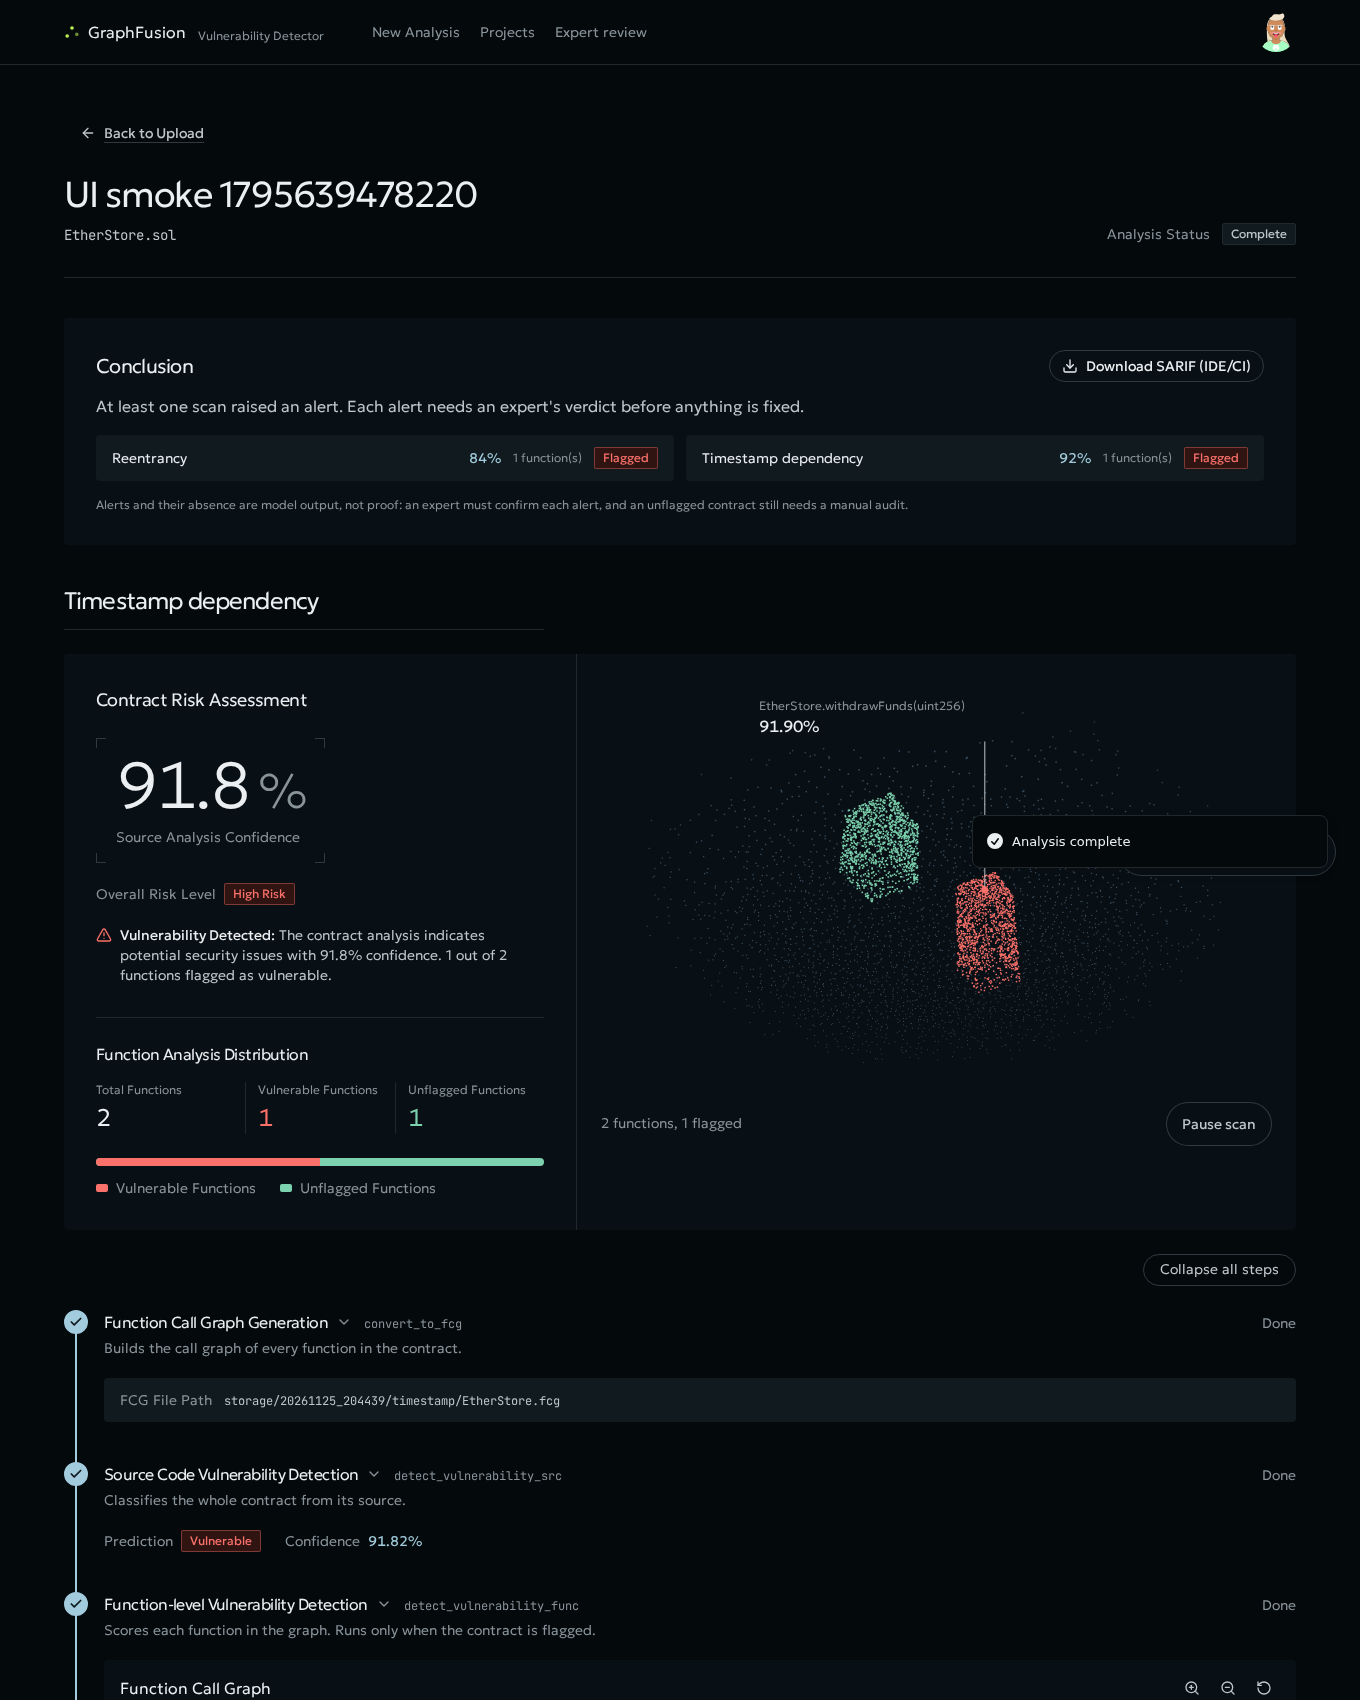
\includegraphics[width=0.82\textwidth]{figures/conclusion-and-scan.png}
\caption{Khối kết luận sau khi hai luồng quét hoàn tất, và chi tiết của một luồng.}\label{fig:conclusion}
\end{figure}

\subsection{Bằng chứng theo dòng mã trong IDE và CI}
\begin{itemize}
\item \textbf{Giải thích có trích dòng.} Với mỗi hàm bị gắn cờ, mô hình ngôn ngữ nhận mã hàm đã đánh số dòng theo file gốc và phải trích đúng dòng làm bằng chứng, nêu tác động, và nêu những gì auditor còn phải kiểm tra. Prompt cấm khẳng định mã an toàn và yêu cầu nói rõ khi cảnh báo có vẻ là dương tính giả.
\item \textbf{IDE trong trình duyệt.} Toàn bộ hợp đồng được mở trong trình soạn thảo, các hàm bị gắn cờ được tô trên đúng dòng, kèm lời giải thích khi rê chuột và ô để chuyên gia ghi kết luận (Hình~\ref{fig:ide}).
\item \textbf{CI và IDE bên ngoài.} Mỗi phiên phân tích xuất được ra SARIF 2.1.0, mở được trong VS Code và GitHub code scanning. Mỗi lỗ hổng có quy tắc riêng (\code{GFD-TS-*}, \code{GFD-RE-*}); mỗi kết quả mang dòng bắt đầu và kết thúc, kết luận của chuyên gia và trạng thái trong quy trình. Cảnh báo bị chuyên gia bác vẫn nằm trong file ở dạng đã suppress để lưu vết. Kho mã có sẵn một GitHub Action mẫu (\code{integrations/github-actions/scanguard.yml}).
\end{itemize}

\begin{figure}[H]\centering
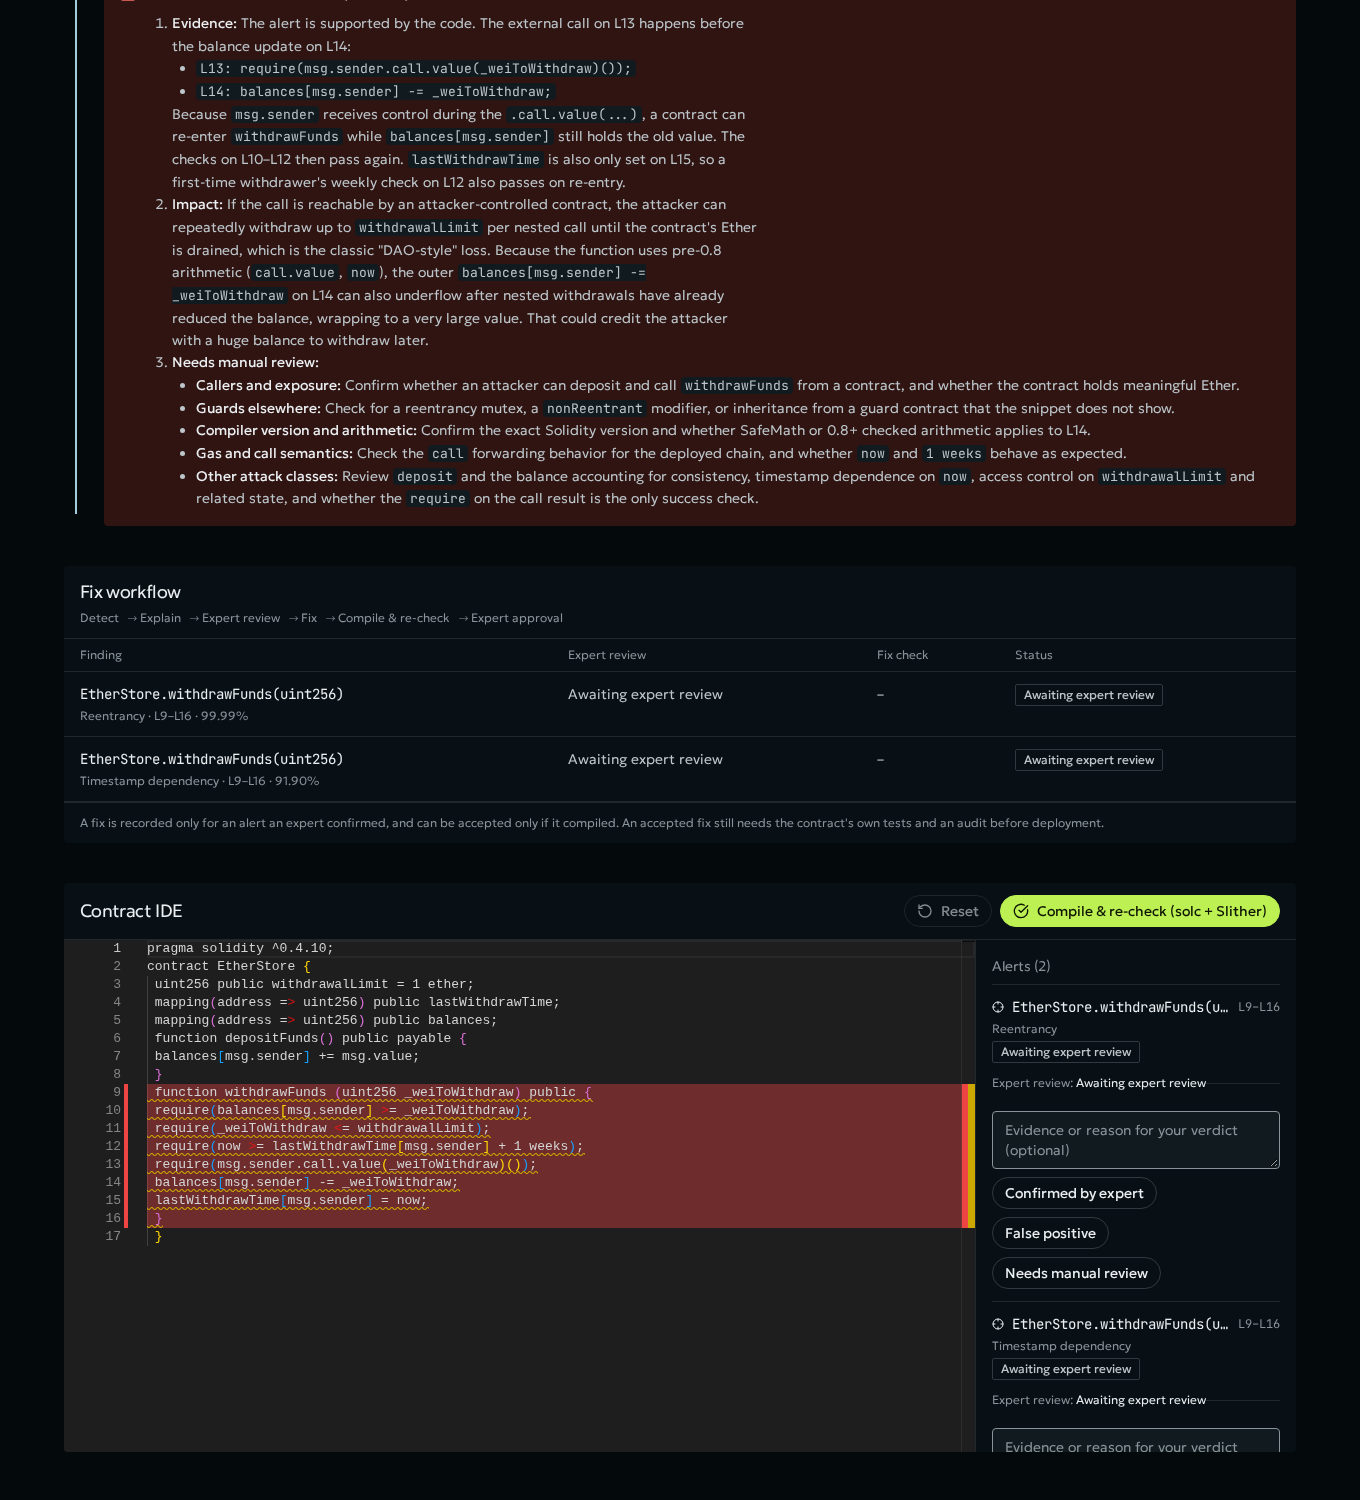
\includegraphics[width=0.82\textwidth]{figures/workflow-and-ide.png}
\caption{Lời giải thích có trích dòng, bảng quy trình sửa lỗi và IDE với hàm bị gắn cờ.}\label{fig:ide}
\end{figure}

\subsection{Vòng đời của một cảnh báo}
Một cảnh báo được định danh bằng cặp (lỗ hổng, hàm), nên cùng một hàm bị hai luồng gắn cờ sẽ được xét riêng.
\begin{table}[H]\centering\small
\caption{Bảy trạng thái của một cảnh báo.}\label{tab:stage}
\begin{tabularx}{\textwidth}{lYl}
\toprule
Trạng thái & Bước kế tiếp & Người thực hiện\\
\midrule
Chờ chuyên gia xét & Xác nhận, bác bỏ, hoặc chuyển rà soát thủ công & Chuyên gia\\
Đã đóng: dương tính giả & Kết thúc; vẫn lưu vết trong SARIF & --\\
Cần rà soát thủ công & Ngoài phạm vi tự động & Con người\\
Đã xác nhận, chờ bản sửa & Đề xuất bản sửa (trợ lý sửa mã hoặc sửa tay trong IDE) & Người dùng\\
Bản sửa không biên dịch được & Sửa lại; không thể chấp nhận & Người dùng\\
Bản sửa đã biên dịch, chờ duyệt & Chấp nhận hoặc từ chối đúng bản đã kiểm tra & Chuyên gia\\
Bản sửa được chấp nhận & Chạy bộ test của dự án và audit trước khi triển khai & Chủ dự án\\
\bottomrule
\end{tabularx}
\end{table}

\subsection{Biên dịch và kiểm tra lại bản sửa}
Khi có bản sửa, hệ thống ghép nó vào đúng vị trí hàm trong hợp đồng gốc, biên dịch bằng bản solc theo \code{pragma}, rồi chạy toàn bộ detector của Slither trên bản gốc và bản đã sửa để so sánh số phát hiện trên các dòng của hàm. Kết quả được lưu vào cảnh báo để chuyên gia duyệt đúng bản đã kiểm tra. Thông báo trả về luôn kèm câu: kết quả đạt không chứng minh bản sửa đúng.

\subsection{Quy tắc do máy chủ thực thi}
\begin{table}[H]\centering\small
\caption{Các quy tắc không phụ thuộc vào giao diện.}\label{tab:rules}
\begin{tabularx}{\textwidth}{Yl}
\toprule
Quy tắc & Kết quả khi vi phạm\\
\midrule
Chỉ tài khoản chuyên gia được xác nhận hoặc bác bỏ cảnh báo & HTTP 403\\
Mọi tài khoản được đề xuất và kiểm tra bản sửa; chỉ chấp nhận được bản sửa của cảnh báo đã xác nhận & HTTP 409\\
Chỉ chuyên gia được quyết định về bản sửa & HTTP 403\\
Chỉ chấp nhận được bản sửa đã biên dịch thành công & HTTP 409\\
Kiểm tra một bản sửa mới thì quyết định cũ bị huỷ & Trở về trạng thái chờ duyệt\\
\bottomrule
\end{tabularx}
\end{table}

\subsection{Demo: phát hiện, giải thích, sửa, biên dịch và duyệt}
Demo chạy bằng \code{demo/run\_demo.py} trên hợp đồng \code{demo/EtherStore.sol}; bản ghi đầy đủ ở \code{demo/transcript.txt}. Script dừng với mã lỗi nếu một quy tắc ở Bảng~\ref{tab:rules} không được thực thi.
\begin{enumerate}
\item \textbf{Phát hiện.} Hai luồng chạy song song. Timestamp: hợp đồng bị gắn cờ (92\%), hàm \code{withdrawFunds} dòng 9--16. Reentrancy: hợp đồng bị gắn cờ (84\%), cùng hàm, xác suất 99{,}99\%.
\item \textbf{Giải thích.} Với reentrancy, lời giải thích trích dòng 13 (lời gọi ngoài) đứng trước dòng 14 (cập nhật số dư). Với timestamp, nó trích dòng 12 (giới hạn rút theo tuần).
\item \textbf{Chặn thao tác sai quyền.} Người dùng thường thử xác nhận cảnh báo: bị từ chối (403). Người dùng thường vẫn được đề xuất và kiểm tra bản sửa trước khi có chuyên gia: bản sửa biên dịch được và được lưu, nhưng cảnh báo vẫn ở trạng thái chờ chuyên gia xét.
\item \textbf{Chuyên gia xét.} Cảnh báo reentrancy được xác nhận. Cảnh báo timestamp bị đánh dấu dương tính giả, vì độ lệch vài giây của thời gian khối không ảnh hưởng tới giới hạn một tuần.
\item \textbf{Sửa và biên dịch.} Một bản sửa hỏng không biên dịch được với solc 0.4.10; chuyên gia thử chấp nhận thì bị từ chối (409). Bản sửa đúng (cập nhật số dư trước khi chuyển tiền) biên dịch được và được lưu.
\item \textbf{Duyệt.} Người dùng thường thử chấp nhận: bị từ chối (403). Chuyên gia chấp nhận.
\item \textbf{Kết quả.} Reentrancy: bản sửa được chấp nhận. Timestamp: đã đóng, dương tính giả. SARIF ghi mức \code{error} cho cảnh báo đã xác nhận và \code{note} kèm suppress cho cảnh báo bị bác.
\end{enumerate}

\begin{figure}[H]\centering
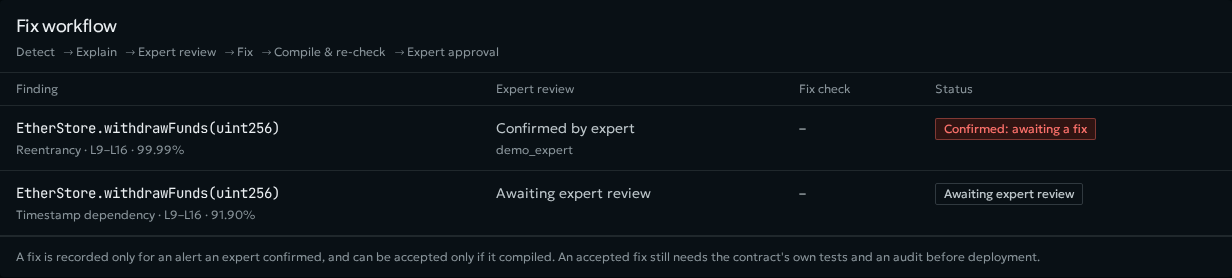
\includegraphics[width=0.9\textwidth]{figures/workflow-after-confirm.png}
\caption{Bảng quy trình sau khi chuyên gia xác nhận cảnh báo reentrancy; cảnh báo timestamp trên cùng hàm vẫn chờ xét.}\label{fig:workflow}
\end{figure}

\subsection{Các trường hợp phải rà soát thủ công}
\begin{enumerate}
\item Hợp đồng không biên dịch được hoặc thiếu file import: luồng quét báo thất bại kèm lý do. Đã kiểm thử bằng một hợp đồng sai cú pháp.
\item Hợp đồng bị gắn cờ nhưng không hàm nào được định vị. Đã kiểm thử: với \code{simple\_dao.sol}, luồng timestamp rơi vào trường hợp này trong khi luồng reentrancy định vị được hàm \code{withdraw}.
\item Chuyên gia chọn \emph{cần rà soát thủ công} cho một cảnh báo hoặc một bản sửa.
\item Không có cảnh báo nào: giao diện và SARIF ghi rõ đây không phải bằng chứng an toàn.
\item Bản sửa đã được chấp nhận: vẫn cần bộ test của dự án và audit trước khi triển khai.
\end{enumerate}

\subsection{Kiểm thử và giới hạn}
Bộ unit test gồm 24 ca đều đạt, trong đó có các ca cho kết luận tổng hợp, vòng đời cảnh báo, SARIF hai lỗ hổng và bước loại comment. Giao diện được kiểm thử bằng trình duyệt tự động trên trang phân tích trực tiếp và trang hàng đợi của chuyên gia.

Giới hạn: bước kiểm thử hiện gồm biên dịch và Slither; hệ thống chưa chạy bộ test riêng của dự án người dùng. Hợp đồng demo nằm trong tập huấn luyện, nên demo minh hoạ quy trình chứ không chứng minh độ chính xác của mô hình.

\section{Kết luận}
\begin{itemize}
\item Trên tập kiểm thử chuẩn, GFD vượt công cụ phân tích tĩnh ở cả hai lỗ hổng, và bước fine-tune CodeBERT theo từng lỗ hổng là thành phần đóng góp rõ nhất.
\item Ngoài tập chuẩn, mô hình còn bỏ sót và cảnh báo nhầm đáng kể, nhất là reentrancy trên mã Solidity mới. Một điểm yếu trước mã đối kháng đã được khắc phục và đo lại.
\item Vì các giới hạn đó, sản phẩm được thiết kế như công cụ hỗ trợ chuyên gia: bằng chứng theo dòng mã, xác nhận bắt buộc của chuyên gia, biên dịch và kiểm tra lại bản sửa, và không khẳng định an toàn tuyệt đối.
\end{itemize}

\end{document}
